% GECCO full paper: at most 8 pages excluding references (ACM acmart, sigconf).
% The GECCO 2027 call still repeats the 2026 text as checked on 5 October 2026;
% recheck the page limit and template instructions before submission.
% Build with: latexmk -pdf -interaction=nonstopmode -halt-on-error main.tex
% main.tex is the anonymous, line-numbered submission version GECCO requires.
% named.tex builds the same paper with author names and no line numbers.
\ifdefined\namedversion
\documentclass[sigconf,dvipsnames]{acmart}
\else
\documentclass[sigconf,dvipsnames,anonymous,review]{acmart}
\fi

%% Rights metadata are placeholders; ACM supplies the real values on acceptance.
\setcopyright{acmlicensed}
\copyrightyear{2027}
\acmYear{2027}
\acmDOI{XXXXXXX.XXXXXXX}
\acmConference[GECCO '27]{Genetic and Evolutionary Computation Conference}{July 12--16, 2027}{Krak\'{o}w, Poland}
\acmBooktitle{Genetic and Evolutionary Computation Conference (GECCO '27), July 12--16, 2027, Krak\'{o}w, Poland}
\acmISBN{978-X-XXXX-XXXX-X/2027/07}

\usepackage{algorithm}
\usepackage{algpseudocode}

\newcommand{\rosarl}{ROSARL}
\newcommand{\pp}{\,pp}

\begin{document}

\title{Evolution Cheats Imagination: Selection Pressure Amplifies Safety Errors in a Learned World Model}

\author{Sachin Mohan}
\affiliation{\institution{University of the Witwatersrand}\city{Johannesburg}\country{South Africa}}
\email{2699183@students.wits.ac.za}
\author{Geraud Nangue Tasse}
\affiliation{\institution{University of the Witwatersrand}\city{Johannesburg}\country{South Africa}}
% Corresponding-author details should be confirmed before a camera-ready version.
\renewcommand{\shortauthors}{Mohan and Nangue Tasse}

\begin{abstract}
Learned world models let evolutionary search evaluate thousands of controllers
cheaply and without physical risk. But selection rewards whatever scores best,
including controllers that exploit the model's errors. We measure this effect
for safety. In Walker2d, we evolve residual controllers inside a frozen visual
world model and replay every selected controller from the same saved simulator
states. In a prospectively locked study (20 paired seeds, four methods, three
population sizes, 320 fresh evaluation episodes), increasing search pressure
widened the gap between actual and imagined failure by 10.39 percentage points
(adjusted 97.5\% interval 6.70 to 14.25). Adding calibrated latent noise and a
\rosarl{}-style return-range penalty reduced this widening by 7.22 points (2.49
to 12.18) and cut actual failures at high pressure from 29.56\% to 22.36\%,
retaining 99\% of forward progress. Yet the starting controller failed on only
16.88\% of the same episodes: the fix limits the damage search does but does not
make search beneficial. Exploratory diagnostics on 89 fixed candidates reveal
both one-step error and rollout accumulation. A subsequent predictor repair
raises failure-endpoint detection from 11.3\% to 67.7\% on a reused audit split,
but its selected controller fails on 3 of 24 branches versus 2 for the starting
controller. Better local prediction does not yet yield better policy selection.
\end{abstract}

\begin{CCSXML}
<ccs2012>
<concept>
<concept_id>10010147.10010257.10010293.10011809</concept_id>
<concept_desc>Computing methodologies~Bio-inspired approaches</concept_desc>
<concept_significance>500</concept_significance>
</concept>
<concept>
<concept_id>10010147.10010257.10010258.10010261</concept_id>
<concept_desc>Computing methodologies~Reinforcement learning</concept_desc>
<concept_significance>300</concept_significance>
</concept>
</ccs2012>
\end{CCSXML}
\ccsdesc[500]{Computing methodologies~Bio-inspired approaches}
\ccsdesc[300]{Computing methodologies~Reinforcement learning}

\keywords{neuroevolution, world models, surrogate models, reality gap, safe reinforcement learning}

\maketitle

%% ===========================================================================
\section{Introduction}
\label{sec:intro}

Evolutionary algorithms need many evaluations. For a robot controller, each
real evaluation is slow, and an unsafe candidate may fall over or damage the
hardware. A learned world model offers a way out: evaluate candidates inside
the model's predictions instead, where trials are cheap and failure costs
nothing~\cite{ha2018worldmodels}. The world model then plays the role of a
\emph{surrogate} fitness function~\cite{jin2011surrogate}.

Every surrogate is wrong somewhere, and selection is drawn to exactly those
places. If a model wrongly predicts that a risky gait stays upright, that gait
scores well, and the best of many candidates is disproportionately likely to be
one the model overrates. Decision analysts call this the optimizer's
curse~\cite{smith2006optimizer}; evolutionary roboticists know it as the reality
gap~\cite{jakobi1995noise,koos2013transferability}. Ha and Schmidhuber's
controller, evolved in a learned ``dream'', scored far higher there than in the
real game until they made the dream noisier~\cite{ha2018worldmodels}. For safety,
the consequence is specific: the controllers evolution selects look safe in
imagination but fail when executed.

This paper asks two questions. \emph{First, how much does selection pressure
widen the gap between imagined and actual safety?} \emph{Second, can two simple
changes to fitness evaluation reduce that widening without sacrificing task
performance?} The changes are Gaussian noise on the model's latent predictions,
scaled to its measured one-step error, and a return-range violation penalty
adapted from \rosarl{}~\cite{tasse2026simple}. Neither ingredient is new; our
contribution is a controlled measurement of what they do, and fail to do, under
evolutionary selection.

We study a Walker2d robot whose controller sees only rendered images. A frozen
LeWorldModel (LeWM)~\cite{maes2026lewm} predicts how its latent visual state
evolves under candidate actions, and separable CMA-ES~\cite{ros2008sep} evolves
a residual correction to a frozen starting controller. Every selected
controller is replayed in the MuJoCo simulator from the same saved states used
in its imagined evaluation (Figure~\ref{fig:walker}), so imagined and actual
outcomes are paired.

Our contributions are:
\begin{itemize}
\item \textbf{A measurement of model exploitation for safety.} In a study
locked before any evaluation data were collected, stronger search widened the
actual-minus-imagined failure gap by 10.39 percentage points (pp), with
adjusted 97.5\% interval $[6.70, 14.25]$.
\item \textbf{A test of a simple mitigation.} Noise plus penalty reduced that
widening by 7.22\pp{} $[2.49, 12.18]$ and lowered actual failures by 7.20\pp{}
at high pressure while retaining 99\% of forward progress. Even so, the
mitigated controllers failed more often than the starting controller.
\item \textbf{A diagnosis and bounded repair of prediction error.} Exploratory
controls separate action feedback, one-step prediction and rollout accumulation.
Predictor-only adaptation improves failure-endpoint detection across three
fitting seeds, but does not improve the real safety of its selected controller.
These follow-ups reuse development episodes and are distinct from the locked
main study.
\end{itemize}

\begin{figure}[t]
\centering
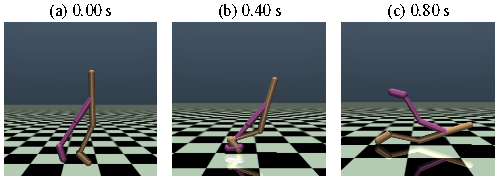
\includegraphics[width=\linewidth]{figures/walker_example.pdf}
\caption{A controller selected by unpenalised, noiseless search, replayed from
saved simulator states. The world model predicted no violation over the
0.8\,s branch, but the simulator records one at step 62 (0.496\,s). This is the
first such example for the first search seed at high pressure, chosen for
illustration rather than as a representative case.}
\Description{Three Walker2d images at 0, 0.4, and 0.8 seconds show an actual
trajectory whose imagined evaluation missed a health violation.}
\label{fig:walker}
\end{figure}

%% ===========================================================================
\section{Related Work}
\label{sec:related}

\paragraph{Reality gaps and surrogates in evolutionary computation.}
Evolutionary robotics met this problem early. Jakobi et al.\ showed that
controllers evolved in simulation transfer better when the simulator is
noisy~\cite{jakobi1995noise}, and the transferability approach adds a
learned estimate of how well simulated fitness predicts reality as a further
objective~\cite{koos2013transferability}. Surrogate-assisted evolutionary
computation replaces expensive evaluations with learned
models~\cite{jin2011surrogate}, and optimization under noisy or approximate
fitness is well studied~\cite{jin2005uncertain}. Specification gaming, where
evolution satisfies the letter of a fitness function rather than its intent, is
widely documented~\cite{lehman2020surprising}. We study the same pressure for a
safety constraint, with a learned visual world model as the surrogate.

\paragraph{Evolution and planning in learned models.}
Ha and Schmidhuber evolved compact controllers inside a recurrent world model
and used a stochastic ``temperature'' to curb exploitation~\cite{ha2018worldmodels}.
Recent audits of action-sequence proposals report that larger proposal pools can
worsen outcomes under latent prediction error~\cite{li2026asar}. Guided Safe
Shooting plans with MAP-Elites in a learned model under safety
constraints~\cite{paolo2022guss}, and SafeDreamer combines world-model planning
with Lagrangian methods~\cite{huang2024safedreamer}. These works plan action
sequences or train with gradients; we evolve the parameters of a closed-loop
controller and measure how selection pressure changes the safety gap.

\paragraph{Model exploitation in model-based RL.}
Gradient-based methods guard against exploiting model error by limiting rollout
length~\cite{janner2019mbpo}, penalising uncertainty in the
reward~\cite{yu2020mopo}, or sending uncertain states to an absorbing failure
state~\cite{kidambi2020morel}. For constrained problems, CAP inflates predicted
costs according to model uncertainty~\cite{ma2022cap}. Our noise is cruder: one
fixed scale per latent coordinate, not a state-dependent uncertainty estimate.

\paragraph{Constraint handling and safe RL.}
Evolutionary computation handles constraints with penalties, feasibility rules
and related techniques~\cite{coello2002constraint,deb2000constraint}. Safe RL
usually formulates safety as a constrained Markov decision
process~\cite{altman1999cmdp}. \rosarl{} instead encodes safety in the reward,
assigning violations a penalty derived from the range of task
values~\cite{tasse2026simple}. We use an evolutionary adaptation of that rule;
its theoretical guarantees do not transfer to our setting.

%% ===========================================================================
\section{Method}
\label{sec:method}

\subsection{Task and safety constraint}

The robot is the Walker2d model underlying
\texttt{SafetyWalker2d\allowbreak Velocity-v1}~\cite{ji2023safetygym}. Instead of that
benchmark's velocity cost, we use a \emph{health} constraint: the torso height
must stay strictly between 0.8 and 2.0\,m and its pitch between $-1$ and
$1$\,rad. A simulator step lasts 8\,ms. We evaluate controllers on short
\emph{branches} of 100 steps (0.8\,s), each starting from a saved simulator
state taken from a recorded episode. A branch \emph{fails} if any of its 100
steps violates the constraint. We disable termination during branches so that
post-failure states and progress are still recorded. Throughout, ``actual''
means execution in MuJoCo, not on physical hardware.

\subsection{World model and controller}

We reuse a previously trained Walker2d LeWM~\cite{maes2026lewm} without
modification. Its encoder maps a rendered image to a 192-dimensional latent
$z$. Its predictor maps the last three latents and actions to the next latent,
one \emph{block} (10 simulator steps, 80\,ms) ahead. Small probes, also
frozen, read torso height, pitch and forward speed from a latent.

The \emph{starting controller} is a frozen ensemble of six networks that map
visual history to actions, trained by imitation of PPO and PPO-Lagrangian
agents. At each block it outputs ten six-motor actions, one per simulator step,
so vision runs at 12.5\,Hz and actuation at 125\,Hz. We evolve only a linear
\emph{residual} added to its output: a $60\times17$ matrix acting on a fixed
16-dimensional projection of the controller's features plus a bias, giving
1,020 parameters. Actions are clipped to $[-1,1]$. The residual starts at zero,
so the initial search distribution is centred on the starting controller.

\subsection{Fitness evaluation in imagination}

To evaluate a candidate, we encode a saved start state's three-frame history
and roll the candidate forward for ten blocks in closed loop: the controller
acts on predicted latents, and the predictor responds to its actions.
Optionally, we perturb each prediction:
\begin{equation}
 z_{t+1}=M(z_{t-2:t},a_{t-2:t})+k\,\sigma\odot\epsilon_t,
 \qquad \epsilon_t\sim\mathcal{N}(0,I).
\label{eq:noise}
\end{equation}
Here $\sigma$ is the per-coordinate standard deviation of one-step
teacher-forced prediction errors (predicted minus encoded latent) on earlier
development data. It is a fixed scale, not a state-dependent uncertainty
estimate. We compare $k\in\{0,1\}$. The perturbed latent feeds the controller,
the probes and all later predictions.

The probes read the predicted state at every block end. Let $v\in\{0,1\}$
indicate an imagined health violation and let $u$ be the imagined forward
progress accumulated strictly before the first violating block (or over the
whole branch if none occurs). We compare two fitness functions, averaged over
start states and noise samples:
\begin{equation}
 F_0=\mathbb{E}[u], \qquad
 F_P=\mathbb{E}\left[u-v\,(V_{\max}-V_{\min})\right].
\label{eq:score}
\end{equation}
Both truncate progress at the first violation; $F_P$ additionally subtracts a
penalty equal to the range of task returns observed so far. Following
\rosarl{}~\cite{tasse2026simple}, the penalty is large enough that no task
return can compensate for a violation, and it requires no hand-tuning.
$V_{\min}$ and $V_{\max}$ are running extrema of $u$ over the search's fitness
evaluations, updated once per generation before ranking. This is a
\rosarl{}-style adaptation, not the original algorithm.

Noise and penalty act together. Because fitness averages over many start states
and samples, it behaves approximately as
$(1-p)\,\bar{u}_{\text{safe}} - p\,(V_{\max}-V_{\min})$, where $p$ is the
candidate's imagined violation rate. Noise raises $p$ for behaviour the model
cannot predict precisely, and the penalty makes a higher $p$ costly.

\subsection{Evolution and selection}

Algorithm~\ref{alg:method} summarises the search. Separable
CMA-ES~\cite{ros2008sep} runs for 16 generations with population size
$\lambda\in\{16,64,256\}$, using coordinates scaled by the inverse RMS of each
projected feature and an initial step size giving an expected unclipped action
change of 0.05 RMS. Each generation evaluates all candidates on 32 start states
drawn without replacement from 96 \emph{fitness} episodes. Noisy evaluation uses
four samples per start state; noiseless evaluation uses one, since it is
deterministic. The best candidate of each generation becomes a \emph{nominee}
and is rescored on 64 fixed \emph{selection} episodes (16 samples per start
state when $k=1$). At generations 1, 4 and 16 we select the best of the starting
controller and all nominees so far. Including the starting controller means
that weak search can, and often does, return it unchanged.

\begin{algorithm}[t]
\caption{Residual evolution in imagination}
\label{alg:method}
\begin{algorithmic}[1]
\Require world model $M$, starting controller $\pi_0$, population size $\lambda$, noise level $k$, fitness $F\in\{F_0,F_P\}$
\State $\mathcal{N}\gets\{\pi_0\}$ \Comment{nominees; residual $=0$}
\State initialise separable CMA-ES at residual $0$
\For{$g=1,\dots,16$}
  \State draw 32 fitness start states
  \State sample residuals $\theta_1,\dots,\theta_\lambda$
  \For{$i=1,\dots,\lambda$}
    \State roll out $\pi_0+\theta_i$ in $M$ with noise $k$ (Eq.~\ref{eq:noise})
  \EndFor
  \State update $V_{\min},V_{\max}$; score candidates with $F$ (Eq.~\ref{eq:score})
  \State update CMA-ES; add best candidate to $\mathcal{N}$
  \If{$g\in\{1,4,16\}$}
    \State \textbf{select} best member of $\mathcal{N}$ on 64 selection states
  \EndIf
\EndFor
\end{algorithmic}
\end{algorithm}

%% ===========================================================================
\section{Experimental Design}
\label{sec:design}

\paragraph{Methods and search pressure.}
Crossing noise ($k=0$ or $1$) with fitness ($F_0$ or $F_P$) gives four methods:
\emph{control} ($k=0$, $F_0$), \emph{penalty}, \emph{noise}, and \emph{noise +
penalty}. Each method runs with 20 search seeds, paired across methods so that
they share random streams and fitness start states, and with all three
population sizes: $20\times4\times3=240$ searches and 720 selected controllers.
We define \emph{low pressure} as population 16 at generation 1 (16 candidates
evaluated) and \emph{high pressure} as population 256 at generation 16 (4,096
candidates evaluated).

\paragraph{Episodes and the locked protocol.}
Start states come from episodes of competent PPO and PPO-Lagrangian agents with
action noise of 0, 0.05 or 0.10, collected until the first violation or 1,000
steps. We take one start state per episode, with enough recorded history and
future for a 100-step branch. This conditions start states on the collecting
agent surviving around them, so our results do not cover arbitrary initial
states. The model, starting controller, noise scale, sample sizes, endpoints and
analysis were locked before we collected 480 fresh episodes, split by episode
seed into 96 fitness, 64 selection and 320 \emph{evaluation} episodes. All 720
selections were frozen before any evaluation outcome was inspected
(Figure~\ref{fig:protocol}).

\begin{figure*}[t]
\centering
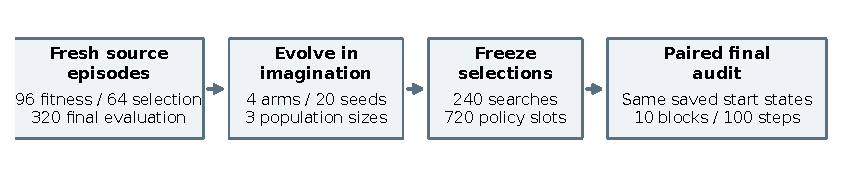
\includegraphics[width=\textwidth]{figures/protocol.pdf}
\caption{Locked study design. Episodes are disjoint across roles, with one
start state per episode. All selections were frozen before final evaluation.
In imagination, controllers act on predicted latents; in MuJoCo, on newly
rendered images. Paired start states therefore do not imply identical action
sequences.}
\Description{A flow diagram links disjoint source episodes, four-method
evolutionary search, a freeze of all 720 selected controllers, and paired final
evaluation.}
\label{fig:protocol}
\end{figure*}

\paragraph{Measurements.}
Each selected controller, and the starting controller, runs from all 320
evaluation start states twice: in imagination ($k=0$, and $k=1$ with 32 samples)
and in MuJoCo. \emph{Actual failure} uses the simulator's health check at every
step. \emph{Imagined failure} uses the probes on predicted latents at block ends.
For method $m$ at pressure $c$, the \emph{gap} is
\begin{equation}
 D_{m,c}=\bar{v}^{\,\text{actual}}_{m,c}-\bar{v}^{\,\text{imag}}_{m,c},
 \qquad A_m=D_{m,H}-D_{m,L},
\end{equation}
with imagined failure measured at the method's own noise level. $A_m$, the
\emph{amplification}, is how much stronger search widens the gap.

\paragraph{Hypotheses and statistics.}
We declared two co-primary contrasts: $A_{\text{control}}>0$ (search widens the
gap) and $A_{\text{noise+penalty}}-A_{\text{control}}<0$ (the combined method
reduces that widening). A smaller gap could simply mean more imagined failures,
so we separately required, at high pressure, that the combined method reduce
actual failure relative to control (95\% interval below zero) while keeping at
least 90\% of its mean forward progress (lower 95\% bound of the ratio above
0.90). Intervals come from 10,000 paired bootstrap replicates that resample
search seeds and evaluation episodes independently, preserving pairing across
methods and pressures. The two primary intervals have 97.5\% coverage each
(Bonferroni family coverage 95\%); all other intervals are descriptive 95\%
intervals. The 6,400 seed--episode pairs per cell are not independent: the
independent units are 20 seeds and 320 episodes.

%% ===========================================================================
\section{Results}
\label{sec:results}

\subsection{Selection pressure widens the safety gap}

Both primary hypotheses were supported (Figure~\ref{fig:primary}). For the
control, the gap grew from 18.70\% at low pressure to 29.09\% at high pressure,
an amplification of $+10.39$\pp{} $[6.70, 14.25]$. Imagined failure barely moved
(0.31\% to 0.47\%), while actual failure rose from 19.02\% to 29.56\%: stronger
search found controllers that looked equally safe to the model but failed
more often. Figure~\ref{fig:pressure} shows the full grid. Larger budgets
generally worsened control safety, but the primary test compares only the
declared endpoints and does not assert monotonicity.

\begin{figure}[t]
\centering
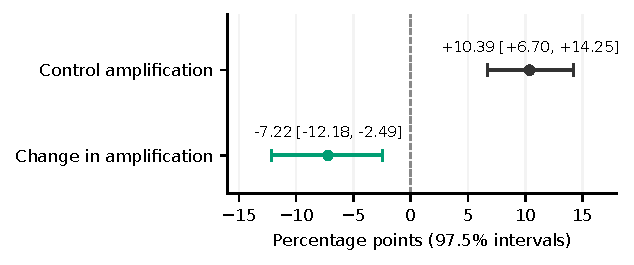
\includegraphics[width=\linewidth]{figures/primary_contrasts.pdf}
\caption{The two co-primary contrasts with 97.5\% intervals. Positive
amplification means stronger search widened the actual-minus-imagined gap;
the negative change means noise + penalty reduced that widening.}
\Description{The control contrast is plus 10.39 percentage points with interval
6.70 to 14.25; the combined-method contrast is minus 7.22 with interval minus
12.18 to minus 2.49. Both intervals exclude zero.}
\label{fig:primary}
\end{figure}

\begin{figure*}[t]
\centering
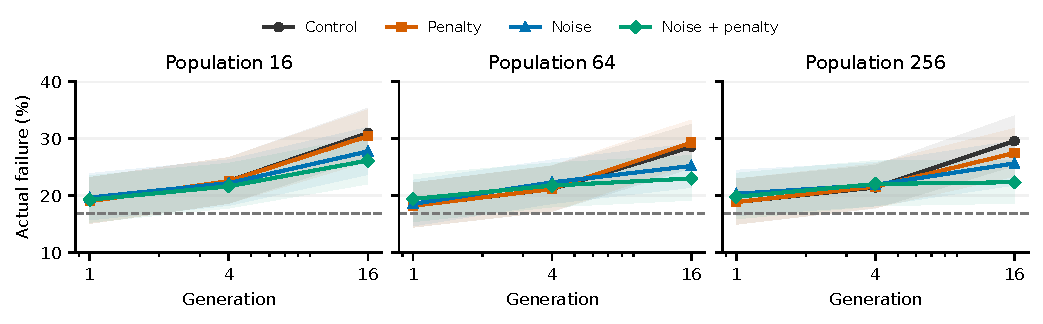
\includegraphics[width=\textwidth]{figures/failure_pressure.pdf}
\caption{Actual failure across all population sizes and generations, with
descriptive pointwise 95\% intervals. The dashed line is the starting
controller (16.88\%). All curves share the same 320 evaluation episodes.}
\Description{Three panels show actual failure rates for four methods over
generations 1, 4, and 16 at populations 16, 64, and 256. Noise plus penalty ends
below the control, while all methods remain above the starting controller.}
\label{fig:pressure}
\end{figure*}

\subsection{Noise and penalty reduce actual failures}

Noise + penalty reduced the amplification by 7.22\pp{} $[2.49, 12.18]$
relative to control. This was not merely a matter of predicting more failures:
at high pressure, the combined method failed on 22.36\% of evaluations versus
29.56\% for control (Table~\ref{tab:main}), a paired difference of $-7.20$\pp{}
$[-10.98, -3.70]$. Its mean forward progress was 2.146\,m versus 2.167\,m, a
ratio of 0.990 $[0.982, 0.998]$. Both practical criteria were met, at the cost
of a small (about 1\%) loss of progress.

Descriptively, both ingredients contributed. At high pressure, adding the
penalty changed actual failure by $-2.09$\pp{} $[-5.39, 0.59]$ without noise and
by $-3.30$\pp{} $[-6.16, -0.48]$ with it; adding noise changed it by $-3.91$\pp{}
$[-7.81, -0.05]$ without the penalty and by $-5.11$\pp{} $[-8.55, -2.02]$ with
it. These secondary intervals are unadjusted and do not establish an
interaction. Noisy search also queries the model four times as often per
candidate, so we have not isolated the effect of noise at equal model compute.

\begin{table}[t]
\caption{Outcomes at high pressure (population 256, generation 16). Imagined
failure uses each method's own noise level; the starting controller's uses
$k=0$. Evolved rates average 20 seeds on 320 shared episodes. Progress includes
post-failure motion.}
\label{tab:main}
\centering
\small
\begin{tabular}{lrrr}
\toprule
Method & Actual (\%) & Imagined (\%) & Progress (m) \\
\midrule
Control & 29.56 & 0.47 & 2.167 \\
Penalty & 27.47 & 0.47 & 2.162 \\
Noise & 25.66 & 5.09 & 2.155 \\
Noise + penalty & 22.36 & 4.95 & 2.146 \\
\midrule
Frozen baseline & 16.88 & 0.31 & 2.141 \\
\bottomrule
\end{tabular}

\end{table}

\subsection{The starting controller remains safer}

The comparison that matters most for deployment is with the controller search
started from. That controller failed on 54 of the 320 evaluation episodes
(16.88\%). The best evolved method still failed 5.48\pp{} $[2.56, 8.44]$ more
often. Even at low pressure, the control was already 2.14\pp{} $[0.67, 4.05]$
worse than the starting controller. Noise and penalty therefore reduce the harm
that optimization causes; they do not make optimization helpful. The imagined
failure rates in Table~\ref{tab:main} are also far below the actual ones (4.95\%
versus 22.36\% for the combined method), so even the noisy model is badly
overconfident.

\subsection{Where the gap comes from}

We split each gap into three parts using two additional readings of every
actual branch: the health check at block ends only, and the probes applied to
encoded \emph{real} images at block ends. (i)~Violations that occur and recover
between block ends contribute only 0.38\pp{} to the control's high-pressure gap.
(ii)~The probes on real images \emph{over}-report violations by 7.27\pp{}, which
narrows rather than widens the gap. (iii)~The remainder, the difference between
the probes on real and on imagined latents, is $+35.98$\pp{}
(Figure~\ref{fig:decomp}). The readout detects more
violations on real images than on imagined latents. This segment-level
decomposition motivates testing the predicted dynamics, but neither establishes
perfect readout accuracy at failure onset nor separates local prediction error
from rollout accumulation. We test those distinctions below.

\begin{figure}[t]
\centering
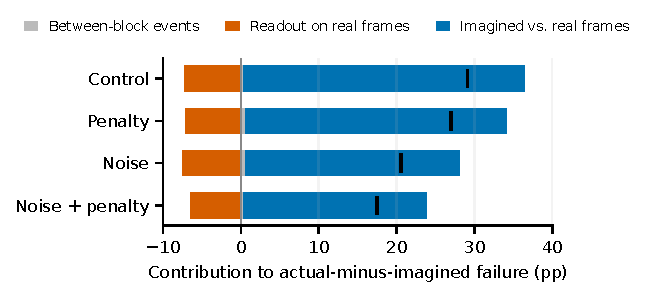
\includegraphics[width=\linewidth]{figures/gap_decomposition.pdf}
\caption{Decomposition of the high-pressure actual-minus-imagined gap. Black
ticks mark the net gap. Nearly all of it arises between probe readings on real
and imagined latents; the probe over-reports violations on real images.}
\Description{Horizontal stacked bars for four methods. A small grey segment
for between-block events, a negative orange segment of about minus 7 points for
the readout on real frames, and a large blue segment of 24 to 36 points for the
imagined versus real frame difference.}
\label{fig:decomp}
\end{figure}

%% ===========================================================================
\section{Exploratory Diagnosis and Model Repair}
\label{sec:diagnostic}

\subsection{Candidate quality}

A natural next step is to check shortlisted candidates in the simulator before
choosing one. In a separate development study (two paired seeds per method),
this simulator-verified selection always returned the starting controller,
because no shortlisted candidate failed strictly less often. That raised a more
basic question: does search produce good controllers that imagination fails to
recognise, or are good controllers simply rare near the starting point?

\paragraph{Design.}
We froze a pool of 89 distinct controllers before any new simulator queries:
the starting controller; the four imagined winners of those development
searches; 32 outcome-blind samples from their populations; 32 random residuals
(eight directions at four scales); and 20 contracted or capped versions of the
winners. Capping clips the difference between the evolved and starting
actions on the same input at every block. All 89 were scored in imagination,
on 32 simulator-selection episodes, and then, after all choices were frozen, on
64 separate check episodes. These episodes had been used in earlier development,
so this audit is exploratory: its intervals are unadjusted and its candidates are
correlated.

\paragraph{Findings.}
On the check episodes, the starting controller failed on 4 of 64. Of the 88
other candidates, 86 failed more often, one tied, and one failed less (3 of 64).
That one candidate had only tied on the selection episodes, so no predeclared
rule would have chosen it. The candidate chosen by simulator selection failed on
6 of 64, rescuing none of the starting controller's failures and adding two. The
candidate chosen by both imagined rankings failed on 12 of 64. Imagination could
not separate the candidates: without noise, \emph{all 89} had zero imagined
failures, and with noise the rank correlation between imagined and actual
failure was 0.04.

Figure~\ref{fig:candidates} shows a clear pattern instead. The further a
candidate moved the starting controller's actions, the more often it failed
(descriptive Spearman correlation 0.78 across this correlated pool). Toned-down
and capped winners failed less than uncapped ones but still more than the
starting controller. For the four controllers whose traces we decomposed (the
starting controller, the one improved candidate, and the two simulator-selected
choices), every actual failure was visible at a block end, and the probes on
real images detected every one of them somewhere in the segment, with two to
five false alarms each. Imagination without noise predicted none. This is
\emph{eventual} detection on four controllers; it does not establish accurate
detection at the first failing endpoint across the complete pool.

\begin{figure}[t]
\centering
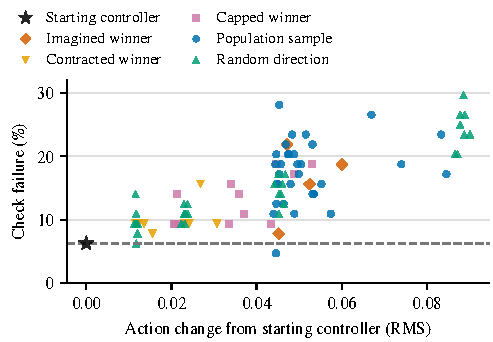
\includegraphics[width=\linewidth]{figures/candidate_quality.pdf}
\caption{Exploratory audit of 89 fixed controllers on 64 reused check episodes.
Failure rises with how far a candidate changes the starting controller's
actions on the same inputs. The dashed line is the starting controller.}
\Description{A scatter plot of check failure against action change. The
starting controller sits at zero change and 6.25 percent failure. Almost all
other candidates lie above it, with failure rising from about 10 percent at
small changes to 20 to 30 percent at the largest changes.}
\label{fig:candidates}
\end{figure}

\subsection{Local prediction error and rollout accumulation}
\label{sec:divergence}

We replayed the saved trajectories through the original predictor, holding the
executed real actions fixed and refreshing its three-frame context from real
latents every one, two, five, or ten blocks. Original closed-loop imagination
provides a fifth path. The refreshes and future action tapes are privileged
retrospective controls. They require no new simulator interaction and are not
deployable root-time predictions.

On the 64 reused check episodes, 861 candidate/episode pairs failed densely.
The block containing the first failure ended unsafe in 819 pairs; 42 transient
events were no longer unsafe at that endpoint. Closed-loop imagination detected
0 of those 819 endpoints, and replaying the exact real actions without refresh
detected only 1. Refreshing real history every block detected 128 (15.6\%),
versus 12.3\% and 2.2\% with refresh every two and five blocks. Different
imagined actions therefore do not explain the misses, and frequent refresh
improves predictions without resolving their local error.

The original probe on real images detected 572/819 first unsafe endpoints
(69.8\%), versus 799/861 failed segments eventually (92.8\%). Thus the readout
also has an onset-detection limitation. These endpoint measurements can follow
the first dense event by up to 72\,ms; they are not advance-warning rates.
Residuals against real-image probe readings exceeded 0.05\,m in height or
0.1\,rad in pitch before nearly all failures, but also somewhere in 71.5\%
of non-failing trajectories with one-step real-history refresh. Residual divergence alone is not a validated failure detector.

\subsection{Predictor repair improves detection, but not controller selection}
\label{sec:repair}

\paragraph{Frozen design.}
We assigned the same 96 previously exposed source episodes to four disjoint
groups of 24 by a fixed hash of episode identity: probe fitting, predictor
fitting, development, and audit. All 89 candidate branches from an episode
stay together. The audit is excluded from fitting and selection in this
procedure, but is reused development evidence rather than fresh confirmation.
We compared the original pipeline, probe-only repair, predictor-only repair,
and both repairs, with three fitting seeds restarted from the original weights.
The encoder, latent projector, action encoder, normalisers and all running
statistics remained frozen. Only the predictor and its output projector, or
the existing same-capacity probe network, received updates.

Each seed used 1,000 AdamW updates per component, batch 256, with predictor/probe
learning rates $10^{-5}/10^{-4}$, weight decay $10^{-4}$ and gradient-norm
clipping at one. Half each batch sampled the last two available endpoints
through a failure-containing block; the other half sampled remaining eligible
endpoints. No later post-failure state was fitted. Probe loss was physical MSE
scaled by $(0.2\,\mathrm{m},0.5\,\mathrm{rad},5\,\mathrm{m/s})$. Predictor loss
was latent MSE plus 0.1 times that physical loss through the original frozen
probe. Targets use detached real latents and privileged simulator labels.

The predeclared one-step development gate required at least a 10\pp{} gain in
first-unsafe-endpoint detection, no more than a 2\pp{} increase in false alarms
at still-healthy endpoints, and at most $1.25\times$ baseline healthy-endpoint
MAE for each of height, pitch and speed. Passing arms were ranked by detection,
then false alarms; the choice was frozen before audit summaries. All intervals
below are descriptive 95\% bootstraps over whole source episodes, conditional
on this candidate pool; fitting seeds and candidate branches are not independent
episodes. Point gates are engineering criteria, not significance tests.

\paragraph{Prediction results.}
Only predictor-only repair passed development, and it also passed audit
(Figure~\ref{fig:repair}). On the audit group's 344 unsafe first-failure
endpoints, mean detection rose from 11.3\% to 67.7\%, a paired gain of
56.4\pp{} $[48.0,61.2]$. The three fitting seeds achieved 69.2\%, 66.0\%, and
68.0\%. False alarms at endpoints strictly preceding dense failure, including
all endpoints on non-failing branches, rose from 0.39\% to 0.85\%. Healthy
height/pitch MAE decreased from 0.02375\,m/0.07903\,rad to
0.02250\,m/0.07571\,rad; speed MAE increased from 0.4462 to 0.4824\,m/s.
Mean height bias at the failure-containing endpoint fell from $+0.1488$ to
$+0.0273$\,m. Without real-history refresh, real-action-tape detection improved
from 0\% to 31.2\%, leaving substantial rollout error. Probe-only repair
achieved 0.9\% one-step detection; combined repair reached 37.3\% but failed
the speed-error retention gate. Better regression of real-image states did not
make that probe reliable on predicted latents.

\begin{figure}[t]
\centering
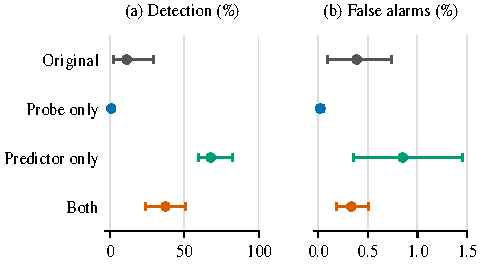
\includegraphics[width=\linewidth]{figures/predictor_repair.pdf}
\caption{Exploratory repair audit: 24 reused source episodes, 89 fixed
candidates. Bars average the three fitting seeds for repaired arms; whiskers
are source-episode bootstrap 95\% intervals. Detection is at the first unsafe
block endpoint, not an advance warning. False alarms use still-healthy
endpoints. Predictor-only repair passes the frozen gate.}
\Description{Two panels compare original, probe-only, predictor-only and
combined repairs. Detection rates are 11.3, 0.9, 67.7 and 37.3 percent;
healthy-endpoint false alarms are 0.39, 0.02, 0.85 and 0.33 percent.}
\label{fig:repair}
\end{figure}

\paragraph{Controller selection.}
We then applied the same imagined-only nomination rule to the original model
and the development-selected repaired predictor: require strictly lower
predicted failure than the starting controller and at least 90\% of its
predicted progress, breaking ties by progress then candidate index. Otherwise
retain the starting controller. All nominations preceded numerical audit
summaries. The original model predicted no baseline failures and fell back to
the starting controller. The repaired model nominated candidate 076, whose
predicted failure was 12.5\% versus the starting controller's 18.1\%.
On the separate audit group, this candidate failed on 3/24 branches versus
2/24 for the starting controller, retaining 98.3\% of actual progress. The
paired failure difference was $+4.17$\pp{} $[0,12.5]$. This small reused audit
does not establish general worsening, but provides no evidence of a controller
improvement. No controller parameters were retrained and no nominee was promoted.

%% ===========================================================================
\section{Discussion and Limitations}
\label{sec:discussion}

\paragraph{What the results show.}
Evolution in a learned world model behaves like optimization against any
imperfect surrogate: more selection finds more of the surrogate's errors, and for
safety those errors are false reports of safe behaviour. Noise and a return-range
penalty push back measurably, but leave a substantial gap. The retrospective
controls expose both one-step errors and their accumulation. Targeted predictor
adaptation improves local failure prediction, yet the resulting model still
misidentifies a beneficial controller in the tested pool. Prediction accuracy
and decision quality require separate evaluation.

\paragraph{Implications.}
First, a smaller imagined-versus-actual gap is not evidence of a safer
controller: the gap can shrink because imagined failures rise. Evaluation must
include actual outcomes. Second, results should be compared with the starting
controller, not only with unmitigated search; against that reference, every
method in the main study made things worse. Third, repairing local prediction
can improve detection without improving selection. The next test should measure
controller-risk rankings over complete closed-loop rollouts, their stability
across source episodes and fitting seeds, and the headroom available in the
fixed pool before another evolution run.

\paragraph{Limitations.}
The main study used one environment, one frozen world model and one starting controller,
on 0.8\,s branches from start states conditioned on survival of the collecting
agent. The starting controller itself fails on a sixth of branches, and earlier
readiness and transfer screens in this project failed; we make no claim of a
safe controller. Development choices, including $k=1$, were informed by earlier
pilots, although the final episodes and analysis were fixed in advance. We did
not test independently pretrained model seeds, full episodes, other environments,
state-dependent uncertainty, or evolution against the simulator itself. The
three repair fitting seeds share the same pretrained model. All follow-ups in
Section~\ref{sec:diagnostic} reuse development episodes and a correlated
candidate pool; their point gates and unadjusted intervals are not fresh
confirmation or safety guarantees. Some upstream costs (agent training, earlier failed runs) are
not fully accounted for.

\paragraph{Cost.}
Table~\ref{tab:costs} separates collection, search and evaluation costs. The
main study ran in 6.8 hours on one GPU with no gradient updates. The main-study
ledger records 26,838,972 simulator steps across 24 preserved runs, plus
3,600,058 shared collection steps for the world model and probes; it is not a
lifetime total. An independent
audit verified all 118 frozen source files and 11,322 query archives and
reproduced the analysis from saved outputs. The later candidate-pool audit
added 854,400 simulator steps and 768,960 predictor rows. The divergence
diagnostic used 427,200 predictor rows. Repair used 768,000 predictor fitting rows,
768,000 probe fitting rows, 3,000 optimiser updates per component across three
seeds, and 320,400 inference predictor rows in 97.2\,s including setup and
writes. The divergence and repair follow-ups used zero new simulator steps, renders
or image encodes;
engineering tests and earlier interaction costs are separate. The repair audit
verified 534 inference archives and three checkpoints. The approved private
archive is not an anonymous public replication package.

\begin{table}[t]
\caption{Main-study compute. A predictor row is one latent transition for one
sample. Final evaluation covers selected controllers, the starting controller
and reference action sequences.}
\label{tab:costs}
\centering
\small
\begin{tabular}{lrr}
\toprule
Phase & Simulator steps & Predictor rows \\
\midrule
Episode collection & 463,921 & 0 \\
Fitness evaluation & 0 & 344,064,000 \\
Selection & 0 & 22,195,200 \\
Final evaluation & 23,104,000 & 78,144,000 \\
\midrule
Total & 23,567,921 & 444,403,200 \\
\bottomrule
\end{tabular}
\end{table}

%% ===========================================================================
\section{Conclusion}
\label{sec:conclusion}

Evolution exploits the errors of a learned world model, and for safety this
means selecting controllers that look safe but are not. In a locked Walker2d
study, stronger search widened the actual-minus-imagined failure gap by 10.4
percentage points. Calibrated latent noise and a \rosarl{}-style penalty
reduced that widening and cut actual failures by 7.2 points at almost no cost in
progress, but every evolved method remained less safe than the controller it
started from. Exploratory follow-ups reveal local prediction error, rollout
accumulation, and imperfect readout at failure onset. Predictor-only repair
raises local endpoint detection substantially but does not improve the real
safety of the selected controller. The next milestone is reliable ranking and
selection of controller risk, followed by fresh confirmation and evaluation
across longer episodes, other robots and independently pretrained models.

\begin{acks}
OpenAI Codex assisted with software development, analysis tooling, manuscript
drafting and figure-generation code. Claude (Anthropic) assisted with revising
the manuscript text and figure code. Numerical figures are generated from saved
experiment outputs; simulator images render saved states. The authors remain
responsible for verifying the text, analysis and references before submission.
\end{acks}

\bibliographystyle{ACM-Reference-Format}
\bibliography{references}

\end{document}
